\documentclass[letterpaper]{article}
\usepackage{natbib,alifeconf}
%Graphics package
\usepackage{graphicx}
\DeclareGraphicsExtensions{.png,.jpg,.pdf}
%For multirow feature to draw tables
\usepackage{multirow}
%Middle allignment in tables.
\usepackage{array}
%For Mathematics
\usepackage{amsmath}
\numberwithin{equation}{section}
%Float package used to specify positioning
\usepackage{float}
%Depth of upto four in sections.
%\setcounter{secnumdepth}{3}
\usepackage{algorithmic}
\usepackage{algorithm}

%For hyper referencing
\usepackage[colorlinks={true},linkcolor={black},citecolor={black},urlcolor={black}]{hyperref}
%In case you use the package hyperref to create a PDF, the links to tables or figures will point to the caption of the table or figure, which is always below the table or figure itself. Therefore the table or figure will not be visible, if it is above the pointer and one has to scroll up in order to see it. If you want the link point to the top of the image you can use the package hypcap with:
\usepackage[all]{hypcap}

\usepackage[acronym]{glossaries}
\makeglossaries
\newacronym{al}{AL}{Artificial Life}
\newacronym{ca}{CA}{Cellular Automata}
\newacronym{cas}{CAS}{Complex Adaptive System}
\newacronym{ea}{EA}{Evolutionary Algorithm}
\newacronym{ec}{EC}{Evolutionary Computation}
\newacronym{ep}{EP}{Evolutionary Programming}
\newacronym{es}{ES}{Evolutionary Strategies}
\newacronym{formal}{FormAL}{Formal Artificial Life}
\newacronym{ga}{GA}{Genetic Algorithm}
\newacronym{gp}{GP}{Genetic Programming}
\newacronym{rna}{RNA}{Ribonucleic Acid}

\title{Modeling the Evolution of Mimicry}
\author{Mohiul Islam$^{1}$ \and Peter Grogono$^{1}$ \\
\mbox{}\\
$^1$Concordia University  \\
moh\_i@encs.concordia.ca \\
grogono@cse.concordia.ca}


\begin{document}
\maketitle

\begin{abstract}
A novel agent based, artificial life model, for the evolution of mimicry is presented. This model is a predator-prey co-evolution scenario where pattern representation phenotype is simulated with Cellular Automata, while behaviors of pattern recognition is configured with Hopfield Network. A visual three dimensional toroidal cube is used to construct a universe in which agents have complete freedom of mobility, genetic representation of behavior and reproduction capability to evolve new behaviors in successive generations. These agents are classified into categories of predator and prey species. Genome of prey species control their mobility and palatability, while 2D Cellular Automata (CA) is used to represent a pattern, where the rule to generate the CA is also genetically represented. Through evolution, successive generations of prey species develop new patterns to represent them both visually and to the predators. Predators are agents with the primary purpose of providing selection pressure for the evolution of mimicry. They are equipped with Hopfield Network memory to recognize new CA pattern and make intelligent decisions to consume the prey based on their level of palatability. Using the above construction of ideas, successful emulation of the natural process of mimicry is achieved. Also complex behavior pattern of Batesian and Mullerian mimicry is simulated and studied.
\end{abstract}

%Introductory Section
\section{Introduction}
\label{section:introduction}

%A few paragraphs are required to bring an appropriate introduction.
Mimicry is a process of deception. It is an evolutionary process with the help of which organisms survive by deceiving its predator. But this deception happens only if the environment contains similar appearing noxious organisms which the predators find unpalatable. Palatable organisms mimic the unpalatable ones through the process of evolution for survival of its species. The objective of this paper is to present an agent based artificial life model for simulating the natural process of the evolution of mimicry.

According to Langton, Artificial Life is `\textsl{Life made by Man rather than by Nature'}. Taylor also defines it as a tool for biological inquiry \citep{taylor1993}. While providing a brief survey over different AL models he talks about \textsl{Wetware systems} which work at the molecular level, the \textsl{Software systems} which work at the cellular level and the \textsl{Hardware systems} which works at the organism level. The initial contribution of \textsl{software systems} in artificial life was from John von Neumann when he designed the first artificial-life model (without referring to it as such), the famous self-reproducing, computation-universal cellular automata \citep{neumann1966}. He tried to understand the fundamental properties of living systems, especially self-reproduction and the evolution of complex adaptive structures, by constructing simple formal systems that exhibit those properties.

Being a special case of complex systems, \gls{cas} are diverse and made up of multiple interconnected elements and adaptive as they have the capacity to change and learn from experience. Echo is a class of simulation model for complex adaptive system, designed primarily for gedanken experiments rather than precise simulations. Echo provides a population of evolving, reproducing agents distributed over a geography, with different inputs of renewable resources at various sites. Each agent has simple capabilities - offense, defense, trading and mate selection - defined by a set of chromosomes. Even though these capabilities are simple and defined simply, they provide a rich set of variations illustrating the four kernel properties of complex adaptive systems described by Holland \citep{holland1996}.

In developing Echo using Holland's criterion, a step by step approach has been taken. Among these steps of improvement, the work by Hraber \citep{hraber1997} is more from an ecological perspective, having a good resemblance with natural ecosystem. 

\section{The Inspiration: Mimicry}
\label{section:mimicry}

Henry W. Bates first published in 1862 his findings about the similarities and dissimilarities between Heliconiinae and Ithomiinae butterflies, after 10 years of research in the Brazilian rain forest. For the next hundred years, it simulated heated discussion among all groups of people, scientists, philosophers, theologians, teachers and amateur naturalists. Bates collected ninety-four pieces of butterfly. He grouped them according to their similar appearance. He found butterflies having similar appearance, exhibiting morphological features which point to completely different species even families. Out of the ninety four species, sixty seven are now classified as Ithomiinae, while twenty seven of them are Heliconiinae.

\subsection{Batesian Mimicry}
Even though Heliconiids are conspicuously colored, they are extremely abundant. They are also slow in mobility. Still predators in the surrounding area, mostly insectivorous birds do not prey on them, because of their inedible and unpalatable nature. Also because of this phenomenon other edible and palatable species such as ithomiinae and pieridae, pretend to be heliconiids and thus enjoy protection.

Repulsive animals, such as heliconiids are very conspicuously colored. Having this noticeable property, they are easily recalled by predators. Their wing pattern works as a warning to predators. Once a predator has the knowledge of their inedible and unpalatable property, they would probably never attempt to try it again. As this is true, if any organism within close family and species, but being edible and having a deceptive resemblance to those conspicuously colored species will be avoided by the predators. 

In general, the animal which is avoided by predator for unpalatable behavior is called the \textbf{model} and the imitating animal is called the \textbf{mimic}.

\subsection{Mullerian Mimicry}
\label{subsec:mullerian-mimicry}
Bates was not able to explain some phenomena of mimicry. Occasionally two inedible unrelated butterfly species are amazingly similar in appearance. An explanation for this was provided by Fritz Muller in 1878. Like Bates, Muller observed and caught butterflies in Brazil. When there are multiple inedible species it is hard for predators to recognize each of them to know which one to consume and which one to avoid. Because of predator's limited memory, all these species still lose their number even after being inedible. So to save this loss, and to prevent more sacrifice of their own kind, inedible species from different family also tend to evolve to have similar appearance. This phenomena is referred to as Mullerian Mimicry in the name of Fritz Muller.

\subsection{Evolutionary Dynamics of Mimicry}
\label{subsec:evolutionary-dynamics-of-mimicry}
The dynamics of mimicry has been investigated by Turner \citep{turner1988}, where he states that the evolution of mimicry can be explained best by the process of punctuated equilibrium instead of phyletic gradualism. 

\paragraph{Punctuated Equilibrium}
In evolutionary biology, punctuated equilibrium is the theory which proposes that most sexually reproducing species will remain in an extended state called \textit{stasis} while experiencing little evolutionary change for most of their geological history. When evolution occurs it is localized in rare, rapid events of branching speciation, called cladogenesis. Cladogenesis is the process by which species split into two distinct species, rather than one species gradually transforming into another. Thus, \textsl{``punctuated equilibria is a model for discontinuous tempos of change (in) the process of speciation and the deployment of species in geological time" \citep{gould1977}}. 

\paragraph{Phyletic Gradualism}
In contrast to punctuated equilibrium, phyletic gradualism states that species continue to adapt to new environmental and biological selection pressures over the course of their history, gradually becoming new species. Phyletic gradualism holds that a species population changes gradually; that is there is no clear line of demarcation between an ancestral species and a descendant species unless a splitting (cladogenetic) event occurs or the gradually-changing lineage is divided arbitrarily. During this process, evolution occurs at a smooth, steady and incremental (but not necessarily constant and slow) rate on a geological time scale. 

To explain the dynamic evolutionary process of mimicry, Turner came up with a synthetic theory \citep{turner1988}, which was originated by Poulton \citep{poulton1912} and Nicholson \citep{nicholson1927}, termed as the \textbf{two stage model}. This theory states that mimicry normally arises in two steps. A comparative large mutation achieves a good approximate resemblance to the model; it is followed by gradual evolutionary changes that refine the resemblance, in many cases to a high degree of perfection \citep{sheppard1972} \citep{ford1964}. This two-stage theory has been applied for the explanation of Mullerian mimicry as well.

\subsubsection{Mimicry Ring}
Any theory of Mullerian mimicry has to take into account the phenomenon of the coexistence of multiple mimicry rings. If we examine the local butterfly fauna in any area of the world, we will find that between all the aposomatic (warningly colored and defended) species present there are normally only a limited number of different patterns, normally far smaller than the number of species. Each cluster of species, all sharing a common pattern, is termed as Mullerian mimicry ring. Thus, in the rain forest of South and Central America, most of the long-winged butterflies (ithomiids, danaids, and heliconids) belong to one of only five different rings.

Like Batesian mimicry, Mullerian mimicry can evolve in two stages: the mutational, one way convergence stage followed by the gradual, mutual convergence stage. It is worth mentioning that in the first stage only the less protected species can adopt the pattern of the better protected species; mutations in the other direction is not favored.

%Chapter describing the model
\section{The Model: Evolution of Mimicry}
\label{section:model}

The agent based artificial life model for simulating the evolution of mimicry, presented in this paper has mainly two species of agents. These agents have properties and behavior similar to the \textbf{model}, the \textbf{mimic} and the \textbf{predator} in the evolution of mimicry. We represent evolution of pattern for the model and the mimic with the help of \gls{ca}. \gls{ca} can be easily represented by simple rules, which can be expressed as a binary string. The predator will be equipped with a Hopfield network \citep{hopfield1982}, to be able to have pattern recognition capability. The process of evolution will of course be running at the genetic level. 

The choice of Hopfield Network memory for a predator can be considered appropriate as the number of patterns which can be recognized by this network is inversely proportional to the accuracy of recall. As more patterns are memorized, Hopfield network tends to make more errors. This behavior will be appropriate for the simulation of Mullerian mimicry. Mullerian mimicry happens because of limited memory of the predators. Because of this limited memory, multiple inedible butterflies seems to converge to a single ring.

The environment is designed as three dimensional, while the space will be of toroidal nature. This idea has been taken from the \textsl{Laws and Life} project by Peter Grogono \citep{grogono2003}.

\subsection{Past Work}
Various models of mimicry has been simulated and explored. The model by Turner \citep{turner1996} and the mathematical model of Huheey \citep{huheey1988} tend to focus on the selective pressure on prey brought about by the particular learning abilities of the predator, and employ simple Monte Carlo or mathematical approaches.

Sherratt \citep{sherratt2002} provides an innovative perspective on the evolution of warning signals by considering co-evolving predator and prey populations. The model's predators are deterministic, in that they have a fixed behavioral strategy over their lifetime, and cannot learn from experience. For both cryptic and conspicuous prey, each predator has fixed policy of either attacking or avoiding.

\subsubsection{Models by Franks and Noble}
\label{subsubsec:models-by-frank-and-noble}
The latest work on modeling evolution of warning signals and mimicry with individual based simulation is done by Franks and Noble. Their initial work \citep{franks2002} seems to focus on putting some conditions of mimetic evolution in an individual based model with multiple species preyed upon by a single abstract predator, where the appearance of each prey species can evolve but their palatability is fixed.

On 2003 \citep{franks2003} another model for the origin of mimicry ring has been proposed by Franks and Noble. This \textbf{second} model is based on two working hypothesis:

\begin{enumerate}
	\item \textsl{All of the Mullerian mimics in a given ecosystem should eventually converge into one large ring in order to gain maximum protection.}
	\item \textsl{If the Mullerian mimics do not converge into one large ring, then the presence of Batesian mimics could entice them to do so, by influencing the rings to converge.}
\end{enumerate}

Although there are many mathematical and stochastic models of mimicry in the biological literature, this model gives attention to the evolution of mimicry ring phenomenon from an artificial life perspective.

Franks and Noble continue to test the influence on mimicry ring evolution by Batesian mimics \citep{franks2004}. Usually mathematical models of mimicry has fixed prey coloration and appearances, which enables a comparison of predation rates to demonstrate the level of protection a mimic might be afforded. In this model prey colorations are free to evolve. This phenomenon is used to examine the effect of Batesian mimicry on Mullerian mimics and mimicry rings.

\subsection{FormAL Framework}
The \textsl{``FormAL framework"} is a collection of ideas and concepts taken from Peter Grogono's \gls{formal} project \citep{grogono2003} and are used to build a framework for modeling the evolution of mimicry. The primary goal of the FormAL project was ``\textit{To study the emergence of complexity}". While the principal behind it was ``\textit{not to include a variable in an agent unless the variable is genetically controlled (or, at least, genetically influenced)}". 

\subsubsection{Agents}
In FormAL, an \textbf{Agent} is a simulated organism. It is designed simply, but with the following qualities:

\begin{itemize}
	\item It has behaviors to be able to reproduce itself using genetic information.
	\item Capable of modifying the structure of genome between generations.
	\item Able to interact with other agents.
	\item And also to survive and reproduce in a challenging environment.
\end{itemize}

\subsubsection{Spatial representation of the environment}
The framework consists of a three dimensional visual environment where agents of the individual based simulation gets complete freedom of movement defined from their genetic representation. 

\paragraph{Space}
The space of the environment is a three-dimensional lattice of discrete points. The coordinate of each point in space is of the form \((x,y,z) \in \Sigma^3\), where \(\Sigma\) be the set \(\{0, 1, ..., S-1\}\). \(S\) is a universal constant being a small positive integer, which in this simulation has been kept at 20 (the value of the \(World Size\) parameter in table \ref{tab:environment-control-parameters}). 

\paragraph{Time}
Time, being an integer \( (t \geq 0) \), advances in discrete steps in the simulation, where at each step the agents update themselves. 

\paragraph{Cell}
The entire three dimensional toroidal environment is divided in multiple cells. A cell is a three dimensional cubical section of the hyperspace. Accordingly in Table \ref{tab:environment-control-parameters} \(ISize\) is the parameter that controls the number of cells in the environment. The size of a cell is evaluated from the entire world size. And the total number of cell is calculated as \(ISize^3 = 216\).

\begin{table}[h]
\small
\centering
\begin{tabular}{| p{1.5cm} | >{\centering} p{1.6cm} | p{4cm} |}
	\hline
		\textbf{Parameter} & \textbf{Value} & \textbf{Description} \\ \hline
		ISize & 6 & Number of cell in single dimension of the 3-D toroidal cube\\ \hline
		World Size & 20 & Size of a single dimension of the 3-D toroidal cube\\ \hline
		Cell Size & \( World Size\) / \(ISize \) & Size of each cell\\ \hline
		Total Number of Cells & \( ISize^3  = 216\) & Total number of cells in the environment\\ 
	\hline
\end{tabular}
\caption{Parameters to control the environment.}
\label{tab:environment-control-parameters}
\end{table}

\subsubsection{Mobility}
An agent's position is calculated once during each step of update in time. The agents \(position\), \(force\), \(acceleration\) and \(velocity\) are all vector components. The \(force\) component is calculated from agent's mobility gene. And it is used to compute agent's \(acceleration\). If the \(force\) and \(velocity\) are both zero, then the agent has no effect in motion. Otherwise, Newton's law is used to obtain the \(acceleration\), which is integrated to obtain the new \(velocity\) and new \(position\).

\subsection{The Prey: Models and Mimics}

Only the significant characteristics which are required for a successful model of mimicry is implemented. As for this simulation we are considering heliconius butterfly, the representation of their wing pattern is with the help of cellular automata. So every prey organism will contain a genetic representation of cellular automata with which the predator will identify the prey and store its level of palatability in memory. We choose cellular automata as it can be easily represented with the help of a binary genome and then evolutionary operations on the genomic representation, such as mutation and crossover can easily be applied.

\subsubsection{Species diversity}
\label{subsubsec:species-diversity}
Franks and Noble have used different models to diversify species. In \citep{franks2002} they have used linear difference in number ``constrained to a 'ring' of values  from 1-20 (where 20 and 1 are neighbors)" to distinguish species diversity. Here the distance of one phenotype from another represents their level of similarity. 

To use CA as prey pattern, an agent's genome is constructed as an 8 bit binary value with a decimal range between 0 to 255. Each of this 256 values have a unique CA pattern associated with it. When storing this pattern in Hopfield memory we take a linear representation of this 2-D pattern, while to consider similarity between two pattern we evaluate the hamming distance between their linear representation. 

With CA based pattern representation, population of prey species with a specific CA pattern can be grouped as one single species. And by restricting inter species reproduction we can control the diversity of patterns. But there is mutation applied when similar species mate with each other, so new species do born out of generations of existing species. That is why we have two separate mutation rate while reproducing prey species. One being the ``Pattern Mutation Rate" (default values are mentioned in table \ref{tab:prey-control-parameters}) with which we control mutation of the first 8 bits of the genome while the ``Genome Mutation Rate" is used to control mutation of rest of the 9 bit genome (table \ref{tab:prey-genome}). Similar efforts of multiple mutation rate at varying location has been used in developing Echo \citep{hraber1997}.

\subsubsection{Genome}
The Genome of the prey species consists of 17 bits as presented in table \ref{tab:prey-genome}. The first eight bits represent the rule, which is used to generate Cellular Automata pattern. The next two bits are used to represent palatability of the organism. The next six bits is the magnitude of the force with which mobility of the organism is calculated. The 17th bit is used to evaluate reproduction capability of the organism, depending on which the prey species is either capable or not capable to participate in reproduction.

\begin{table}[h]
\small
\centering
\setlength\tabcolsep{2pt}
\begin{tabular}{|c|c|c|c|}
	\hline
		\textbf{Pattern(8)} & \textbf{Palatability(2)} & \textbf{Mobility(6)} & \textbf{Reproduction(1)} \\ \hline
		10101101					 	& 							01		 		 & 			110001					&					1						 		 \\ \hline
\end{tabular}
\caption{Distribution and purpose of each gene of the 17 bit prey genome.}
\label{tab:prey-genome}
\end{table}

\subsubsection{Reflection of punctuated equilibrium}
\label{subsubsec:reflection-of-punctuated-equilibrium}
Punctuated equilibrium is more inclined to cladogenesis instead of gradualism. Also Turner \citep{turner1988} emphasizes on punctuated equilibrium to describe the evolution of mimicry instead of phyletic gradualism. The design of the model under discussion also follows Turner's explanation in terms of evolving mimicry. As it can be observed, new CA patterns evolve from existing ones in prey population just by a single mutation in the pattern gene. Mimics do not follow a gradual process of evolution to look close to models but rather the change happens randomly through a single step mutation. The mutations that are favored, helps the mimics to survive while the unfavored ones fail to persist. It can be observed later in table \ref{tab:diff-in-pattern} how CA patterns of prey species can have vastly different configuration for a unit change in their representative gene. 

\subsubsection{Genetic representation of palatability}
\label{subsubsec:genetic-palatability-representation}
The palatability of each prey species is fixed and has been represented with 2 bits of the genome giving it a range of 0 to 3 with four levels of palatability. The combinations are as follows:

\begin{table}[h]
	\small
	\centering
	\begin{tabular}{|c|c|}
		\hline
			\textbf{Gene (Index 8 to 9)} &	\textbf{Palatable} \\ \hline
			00 or 01						& True 			\\ \hline
			10 or 11						& False 		\\
		\hline
	\end{tabular}
	\caption{Genetic representation of palatability}
	\label{tab:genetic-representation-palatability}
\end{table}

This representation in table \ref{tab:genetic-representation-palatability} is unlike Franks and Noble \citep{franks2003} where palatability level has been used on a scale between zero and one (least to most palatable), where 0.5 is neutrally palatable. 

\subsubsection{Interaction between other Prey and Predators}
The prey have been defined to have many conglomerate behavior in the environment. Prey interaction with other prey species and with predators make the evolution of mimicry possible. Mobility of prey species and their reproduction capability are two important behaviors which result from interaction. 

\paragraph{Mobility}
The mobility genes of the prey consist of 6 bits. These six bits are used to calculate the force with which each prey try to move towards any neighborhood cell. The algorithm sorts all neighboring cell descending to the number of prey species. Then it selects the cell which contains the highest number of prey with zero predator. If all the neighboring cells contain predators, then the algorithm sorts the neighboring cells descending on the number of predators and chooses the one which contains the least.

\paragraph{Reproduction}
Every prey species starts reproducing when it reaches the \textsl{``Reproductive age limit"}. If it is capable of reproducing, which is decided based on its 17th bit gene, the prey will randomly select another prey species with similar pattern and palatability from the same cell and mate with it. Now the other prey also needs to be genetically capable of reproduction and needs to reach its age limit. A new genome is created from the existing genome of the two prey by applying single point crossover operation. Mutation is performed separately on the pattern gene and the rest of the genome, with two different rates to control them using the values in table \ref{tab:prey-control-parameters}. So there is two point mutation for the genome. 

\begin{table}[h]
\small
\centering
\setlength\tabcolsep{2pt}
\begin{tabular}{| p{2cm} | p{1cm} | p{5cm} |}
	\hline
		\textbf{Parameter} & \textbf{Value} & \textbf{Description} \\ \hline
		Prey Size & 2 to 5 & Size of the prey species in the 3D FormAL  environment.\\ \hline
		Reproduction age limit & 100 & Minimum number of iterations or time steps a prey species need to be present in the simulation to get reproduction capability\\ \hline
		Reproduction interval & 1000 & Number of iterations a prey need to wait before reproducing again.\\ \hline
		Pattern Mutation Rate & 0.05 & Rate of Mutation of the pattern genome.\\ \hline
		Genome Mutation Rate & 0.5 & Rate of mutation of the rest of the genome excluding the pattern gene.\\ \hline
		Demise Age & 2000 & Age at which the prey species will be removed from the environment.\\
	\hline
\end{tabular}
\caption{Parameters to control prey population and visibility.}
\label{tab:prey-control-parameters}
\end{table}

\subsection{Predator}

Predators in the system are designed to provide selection pressure to \textit{models} and \textit{mimics} for the evolution of mimicry. Similar to prey species, they are agents in the FormAL environment capable of mobility and reproduction. In addition to it, these agents are equipped with Hopfield Network Memory to be able to learn and recognize patterns of the prey species. Their mobility and reproduction capability are controlled at the genetic level, while their memory is not genetically controlled, as it was not possible to come up with a genetic representation for Hopfield Network. So every new predator species gets to born with zero memory and with no inheritance from parents. A set of parameters are defined to control predators' population and learning ability in the environment. Details of which are in table \ref{tab:predator-control-parameters}.

\subsubsection{Learning}
The objective of a predator's interaction with prey is always to consume it. But based on the prey's pattern and palatability, the predator will either be able to consume it or throw it back to the environment. At this event the predator needs to learn the pattern with which the prey has been represented. The pattern represents palatability of the prey species, at least to the predator. Every time a new interaction is made by the predator its memory is initialized with all the existing pattern that has already been encountered and the new one. The learning procedure used for this memory is Hebbian Learning \citep{hebb1949}, which represents a purely feed-forward, unsupervised learning. Initially the weights of the Hopfield Network are all set to zero. Using Hebbian rule, the outer product of the input - output vector pairs are calculated for each pattern. As Hopfield is a feedback network, the output of the network is also the input. The outer vector matrix of all the patterns are summed to come up with the final weight matrix.

%This section needs to use similar variables as mentioned in the above section on Hopfield Network.
\paragraph{Input to memory}
Each prey contains an evolving cellular automata which is represented by a binary genome. This two dimensional pattern is serialized to be available as a one dimensional binary array, which is taken as input for any predator organism trying to interact with the prey. This binary representation of the pattern gets converted to a bipolar representation. Each input pattern consists of \(\textit{m} \times \textit{n} = \textit{mn}\) components, each component representing one pixel of the pattern (\textit{m} and \textit{n} representing each dimension). The \textit{m} by \textit{n} pattern configuration will be serialized by putting all row vectors in one single row sequentially.

\paragraph{Predator attack algorithm}
As soon as a predator reaches its attack age it selects random prey species around its vicinity and starts attacking them. This attack process also involves recognition of prey pattern. Two parameters have been defined to limit predator memorization and recognition process as both of these processes are computationally expensive. The ``Hopfield Minimum Memory Size" is the number of memory a predator needs to store before making intelligent decisions about attacking a new prey species. After a predator is born, it start attacking prey without any caution. But after every attack the predator will store its pattern and palatability level inside its memory. As soon as it reaches the minimum memory size, it will start making intelligent decision about attacking the next species. It will try to recognize the pattern and if found palatable, prey will be consumed. Otherwise prey will be thrown back into the environment. If the pattern is not recognized predator will try to consume it and in the process will store its palatability and pattern into memory. In this way the predator memory is limited to \textsl{``Hopfield Maximum Memory Size"}. After reaching this memory predator will not store any more new pattern but will try to associate with the existing ones it has already stored.

\subsubsection{Genome}
Each predator has a 5 bits genome as explained in table \ref{tab:predator-genome}. The first 4 bits represent its mobility and magnitude of the force component with which it moves around the environment. The last bit controls reproduction capability of each species.

\begin{table}[h]
\small
\centering
\begin{tabular}{|c|c|}
	\hline
		\textbf{Mobility(4)} & \textbf{Reproduction(1)} \\ \hline
				 1101					   &					1						 		\\ \hline
\end{tabular}
\caption{Distribution and purpose of each gene of the 5 bit predator genome.}
\label{tab:predator-genome}
\end{table}

\subsubsection{Mobility and reproduction capability}
Movement behavior of a predator is calculated from its genome. The first 4 bits of the genome are converted from binary to decimal to determine the magnitude of force at which it will move towards the maximum crowd of prey present within its neighborhood. So magnitude of movement of a predator varies within a range of 0-15 units. If no prey is present in the neighborhood then this force is active in trying to keep predators distributed all over the cells. A predator chooses the neighborhood cell which contains the least number of predators. When the neighborhood contains zero predators, it would select any one of them randomly and move towards that cell.

The predators are distributed all over the cells with a constant mobile behavior to switch to another neighboring cell depending on the one containing the least number of predator and also most number of prey species. This behavior of predator has been designed to enforce the predatory capabilities of these agents and also to have increased predator prey interaction in the simulation in terms of one agent chasing the other for survival of species. 

\subsubsection{Reproduction process}
The  fifth gene of the predator is used to represent their capability of reproduction.  Depending on its binary value a predator in the simulation will or will not be able to reproduce. The reproduction process for predators is similar to prey species. As the learning capability of predators do not have any genetic representation, only the mobility behavior and reproduction capability takes effect in the reproductive process from one generation to another. 

There are two control parameters that effect the reproduction of predator species. The first is \textsl{``Reproduction Age Limit"}. This is the minimum age a predator has to reach before starting to involve itself for reproduction. This parameter has been set to 500 iterations. The second parameter is \textsl{``Reproduction Interval"} which has been varied in the simulation from 1000 to 3000 iteration depending on the population of palatable prey species. This is a very important parameter for the simulation as it determines the overall predator population and its rate of increment. Depending on this value we can control the rate of predation on prey species, which on the other hand controls the rate of mimetic behavior of the overall prey population.

\begin{table}[h]
\small
\centering
\begin{tabular}{| l | c |}
	\hline
		\textbf{Parameter} & \textbf{Value} \\ \hline
		Minimum Memory Size & 2 to 6 \\ \hline
		Maximum Memory Size & 10 \\ \hline 
		Hopfield Maximum Iterations & 20 \\ \hline
		Attack Age & 500 \\ \hline
		Attack Interval & 100 \\ \hline
		Genome Mutation rate & 0.3 \\ \hline
		Reproduction Age Limit & 500 \\ \hline
		Reproduction Interval & 1000 to 3000 \\ \hline
		Demise Age & 2000 to 7000 \\
	\hline
\end{tabular}
\caption{Distribution and purpose of each gene of the 5 bit predator genome.}
\label{tab:predator-genome}
\end{table}

This model has been designed to come up with efficient results and achieve the main objective, \textit{evolution of mimicry}. Creation and transformation of different mimicry ring and also the dynamics of it has been integrated to achieve interesting results. This model can also be considered as a complex adaptive system similar to Holland's work on Echo \citep{holland1996}. The seven basics of a complex adaptive system which are: Aggregation, Tagging, Nonlinearity, Flow, Diversity, Internal Models and Building blocks \citep{holland1996} are present in this model. Individual components of this model such as the different types of agents and their properties can be considered as \textit{building blocks}. Each prey species are \textit{tagged} with individual pattern and palatability with which predators recognize them. We are providing different properties, behaviors and goals to the agents but setting them free in the environment to observe their \textit{aggregate} behavior, resulting in \textit{non-linear} or unpredictable outcome. The model has its \textit{flow} as it progresses in time. Also there is \textit{diversity} of prey species in the environment.

\section{The Results}
\label{section:results}

Data and analysis in this simulation has been concentrated on evaluating whether evolution of mimicry has taken place. This evaluation can be made with the number of different rings that has been created and the size of each of those rings along with the population of palatable and unpalatable species. Also it can be established whether Batesian Mimicry and Mullerian Mimicry have taken effect by analyzing the data set of these populations.

\subsection{Mimicry Ring Reports}
The mimicry ring reports consist entirely of the population of prey species categorized according to pattern and palatability. Data is stored for time interval of 10 iterations. As the number of rings that get generated reaches as many as 50 or more, and all the population of ring do not last for the entire simulation, so while storing data we have taken the most populous of the surviving 8 rings to plot. Parameters are mentioned in table \ref{tab:ring-report-control-parameters}.

\begin{table}[h]
\small
\centering
\setlength\tabcolsep{2pt}
\begin{tabular}{| p{2cm} | >{\centering} p{1cm} | p{5cm} |}
	\hline
		\textbf{Parameter} & \textbf{Value} & \textbf{Description} \\ \hline
		Mimicry Ring Hamming Distance & 10 \% of the Pattern Size & If the Hamming distance between the pattern of the model and the mimic is 10 \% the size of the pattern then they are considered within the same ring.\\ \hline
		Number of Rings to report & 8 & This value is the number of most populous rings that are included in the report.\\
	\hline
\end{tabular}
\caption{Parameters to mimicry ring report.}
\label{tab:ring-report-control-parameters}
\end{table}

\subsection{Initial configuration with two prey species}
\label{subsec:init-conf-2prey}
% Put the table here
\begin{table}[h]
\small
\centering
\setlength\tabcolsep{2pt}
\begin{tabular}{| p{2cm} | p{1.5cm} | p{1cm} | p{.5cm} | p{1.5cm} | p{.5cm} |}
  \hline
   														&\multicolumn{3}{c|}{Prey configuration} 																	
   														& \multicolumn{2}{c|}{\parbox{2cm}{Predator \\ configuration}} \\ \hline
  \multirow{2}{*}{Population} & Rule110 (Palatable) & \parbox[c]{2.1em}{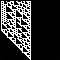
\includegraphics[scale=0.50]{../tex/images/CARule110}} & 108 
  														& \multicolumn{2}{c|}{\multirow{2}{*}{10}} \\ \cline{2-4}
  					 									& Rule30 (Unpalatable)& \parbox[c]{2.1em}{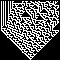
\includegraphics[scale=0.50]{../tex/images/CARule30}}  & 108 
  					 									& \multicolumn{2}{c|}{}\\ \hline
  \multirow{2}{*}{Reproduction} & Age Limit & \multicolumn{2}{c|}{100}  & \multicolumn{2}{c|}{500} \\ \cline{2-6}
  						 									& Interval  & \multicolumn{2}{c|}{1000} & \multicolumn{2}{c|}{1200} \\ \hline
  \multirow{2}{*}{Mutation Rate} & Pattern   & \multicolumn{2}{c|}{0.05} & \multicolumn{2}{c|}{\multirow{2}{*}{0.3}} \\ \cline{2-4}
  						 									 & Genome    & \multicolumn{2}{c|}{0.5}  & \multicolumn{2}{c|}{} \\ \hline
  Demise Age	 									 & \multicolumn{3}{c|}{2000}							& \multicolumn{2}{c|}{2500} \\ \hline
  Minimum Attack Age						 & \multicolumn{3}{c|}{} 						    & \multicolumn{2}{c|}{500} \\ \hline
  \multirow{2}{*}{\parbox{2cm}{Memory Configuration}} & \multicolumn{3}{c|}{} 					& Minimum & 2 \\ \cline{5-6}
   																			& \multicolumn{3}{c|}{} 					& Maximum & 10 \\ \hline  
\end{tabular}
\caption{Agent configuration of 2 prey species}
\label{tab:config-table-2-prey}
\end{table}

The set of parameters in table \ref{tab:config-table-2-prey} were carefully selected to be the initial condition for this run of the simulation. This test has been done with two sets of prey species with very different Cellular Automata pattern and with opposite palatability and equal population. To control reproduction of the prey species their age limit has been set to 100 iterations into the time the species were alive. And the reproduction interval was set to 1000 iterations.

Pattern mutation rate has been set to a minimal level of 0.05 as by increasing this variable it is possible to increase the size of the number of mimicry rings present in the simulation. The genome mutation rate controls the rate at which genome of the child prey species will deviate from their parents. As mentioned earlier the genome mutation rate has been separated from the pattern mutation rate to bring more control to the number of mimicry rings generated.

Prey demise age has been kept to 2000 iterations while predator demise age is set to 2500. But in the later experiments predator demise age has been increased to 5000 iterations. Predators in this simulation generate selection pressure for the evolution of mimicry. So the longer a predator is present in the simulation it will be making intelligent decisions in term of selecting which prey species to consume and which one to avoid. But with the current rate of demise for predator we were able to create successful mimetic population of prey species as we will see in the analysis in the following results.

Initial population of predator species has been set to 10 which is in accordance with the prey population in the simulation. The reason for such low number of predator is, unlike prey species which are consumed by predators, there is no cause for the predator species to die accept their natural cause of death, that is to reach their demise age. So predator population can explode very easily. That is why their population is controlled in a restrictive manner with the help of high reproduction age limit and reproduction age interval.

The memory configuration size for predators is a very interesting parameter. The minimum memory size is directly associated with the number of prey species with which we initiate the simulation. Otherwise evolution of mimicry is not observed. As mentioned in table \ref{tab:predator-control-parameters} the minimum memory size is the number of prey species predator would consume before starting to make decisive consumption of prey species. Based on the behavior of Hopfield memory, a recognition result will always be achieved depending on the similarity of the patterns stored in memory. So when minimum memory size has been reached the predator will always make a decision based on the similarity of the prey pattern currently captured and the patterns stored in memory.

% Put the image
\begin{figure*}[t!]
	\centering
	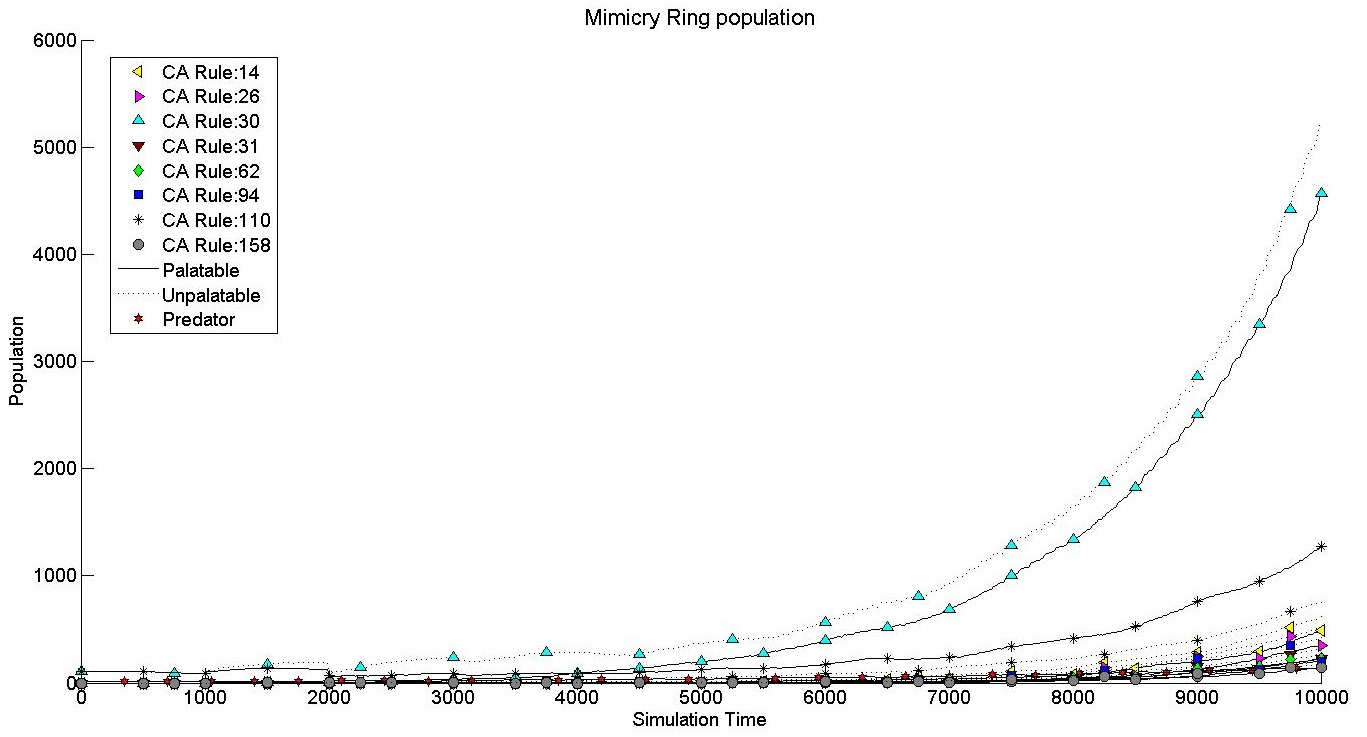
\includegraphics[width=0.75\textwidth]{../tex/images/simTime10k-2Prey}
	\caption[Population distribution of mimicry rings (2 prey species, 10k iterations)]{Population distribution of mimicry rings, initialized with 2 prey species, 10k iterations}
	\label{fig:plot-2-prey}
\end{figure*}

The plot in Figure \ref{fig:plot-2-prey} is simulation time verses prey population after running it for 10000 iterations. With the initial configuration in the above table we can observe that multiple rings of prey population have been created. Two prey species are considered to be in a ring if their CA pattern have a Hamming distance within 10 bits. Population of palatable species has been represented with line curve while population of unpalatable species has been presented with dotted curve. Different signs of squares, triangles and diamonds have been used to distinguish between species of prey population. The simulation was initiated with two prey species having CA rule of 30 and 110 and being palatable and unpalatable consecutively. Over time the population of CA Rule 30 dominates the population (Figure \ref{fig:plot-2-prey}) as most predators recognize it as unpalatable. Similarly a palatable population of CA Rule 30 or within the same ring of palatable species starts rising, while at one point overlaps the population of CA Rule 110 (Time: 4000 approx.). CA Rule 110 was initialized as a set of palatable species.

We can observe from the above result that the evolution of mimicry has taken effect. A population of mimics were successfully able to exceed the population of other prey species, and the reason being, avoidance by predators of prey pattern similar to unpalatable ones. We can conclude that Batesian mimicry has taken effect in the simulation.

%Put the number of rings picture:
\begin{figure}[h]
	\centering
	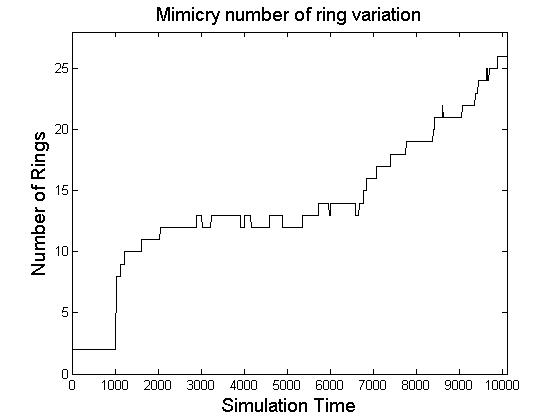
\includegraphics[width=0.4\textwidth]{../tex/images/ringSize10k-2Prey}
	\caption[Number of mimicry rings (2 prey species)]{Number of mimicry rings, initialized with 2 prey species.}
	\label{fig:ringSize10k-2Prey}
\end{figure}

Observing from figure \ref{fig:ringSize10k-2Prey} the number of rings in this simulation makes a slow increase from 2 at the initial configuration to 27 rings at the end of 10000 iterations. A small change in CA genetic representation can have a very large effect in terms of the phenotype of the pattern with which the prey is represented. For example if we take a look at the set of pattern genotype with very different phenotype in table \ref{tab:diff-in-pattern}.

%CARule table
\begin{table}[h]
\small
\centering
\setlength\tabcolsep{2pt}
\begin{tabular}{|l|c|c|c|}
  \hline
  CA Rule & \(60 \equiv 00111100\) & \(61 \equiv 00111101\) & \(62 \equiv 00111110 \) \\ \hline
  Pattern & \parbox[c]{2.1em}{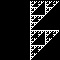
\includegraphics[scale=0.50]{../tex/images/CARule60}} 
  				& \parbox[c]{2.1em}{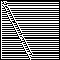
\includegraphics[scale=0.50]{../tex/images/CARule61}} 
  				& \parbox[c]{2.1em}{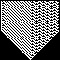
\includegraphics[scale=0.50]{../tex/images/CARule62}}\\
  \hline
\end{tabular}
\caption{Difference in prey pattern genotype and phenotype}
\label{tab:diff-in-pattern}
\end{table}

All the patterns in table \ref{tab:diff-in-pattern} have a genetic bit difference of 1. So by a single mutation there can be three different set of phenotype for a child organism from its parent. This is largely the reason for the increased number of mimicry rings created in the simulation. Only the 8 most populous rings are presented in the graphs with population verses simulation time.

\subsection{Initial population with six prey species}
\label{subsec:init-conf-6-prey}

To evaluate the simulation at a more complex level we increase the prey population to 900, consisting of 6 different species with very different pattern configuration. To boost predator-prey interaction we also increase the number of predator population to 30. Predator reproduction interval has been set comparatively lower in this simulation to 2000 iterations. As the initial population of prey species is very high, over time we are expecting even larger number of prey species. If predator population does not increase at similar rate there might be a prey population explosion were predator will have no effect on providing selection pressure for the evolution of mimicry. So that is why predator population control parameter has been set to this level. For memory configuration, the minimum number is set to 6, meaning the predator will have to store 6 different prey pattern configuration before starting to make intelligent decision about consuming them. As previously mentioned this number is always set in accordance with the initial number of different prey configuration. An enormous diversity of species can be observed from this experiment. In addition to the six prey species with which the simulation starts, the total number of mimicry rings reach nearly 50.

\subsection{Initial configuration with only unpalatable species}
\label{subsec:init-conf-only-unp}

To further observe the effects of mimicry ring we initialize the simulation with all four unpalatable prey species. As explained earlier the minimum memory configuration is also set to four in accordance to the initial number of prey species. Rest of the parameters remain quite unchanged.

\begin{figure*}[t!]
	\centering
	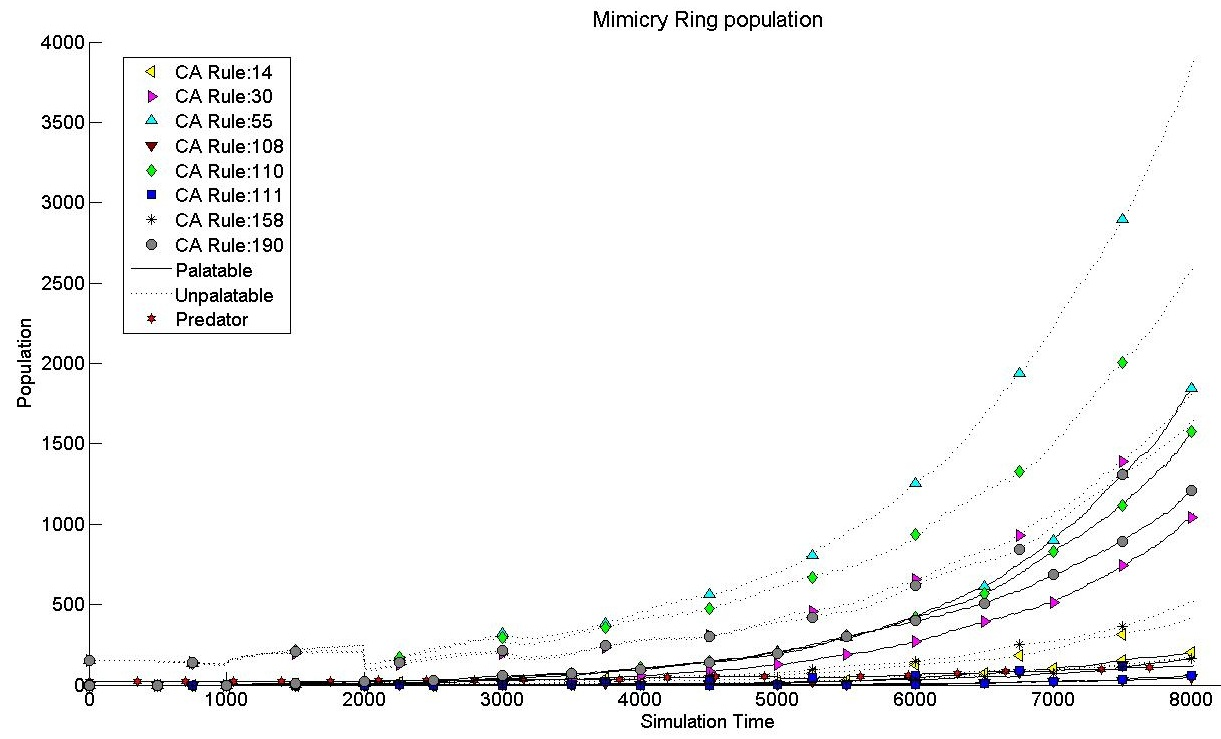
\includegraphics[width=0.75\textwidth]{../tex/images/simTime8k-4Prey-unp}
	\caption[Population distribution of mimicry rings(4 prey species all unpalatable)]{Population distribution of mimicry rings, initialized with 4 prey species all unpalatable.}
	\label{fig:plot-4-prey-unp}
\end{figure*}

The results according to figure \ref{fig:plot-4-prey-unp} are much expected. The population of unpalatable species have prevailed. After nearly 8000 iterations we can see unpalatable species of CA rule 55, 110, 30 and 190 have prevailed with the most population. All of their palatable counter parts are also increasing their population deceiving the predators. We observe the effect of the simulation up to 8000 iterations instead of 10000 as the total number of prey species increases at an enormous rate in this simulation within very short period of time. As most of the species are unpalatable, predators mostly do not get the opportunity to consume, causing a much lower prey death rate. 

This experiment is an ideal scenario for observing Mullerian mimicry. Mullerian mimicry occurs between multiple species of unpalatable prey population. From the second work of Franks and Noble \citep{franks2003} mentioned in section \ref{subsubsec:models-by-frank-and-noble}, we note that multiple Mullerian mimicry rings are expected to converge into one large ring through the evolutionary process of punctuated equilibrium. But in this experiment as the predator's `Minimum Memory Configuration' is set to four, all predators have the capability to recognize four prey patterns before starting to make intelligent decision of consuming them. By setting `Minimum Memory Configuration' to one, also increasing `Predator Demise Age' to 7000 and decreasing predator's `Reproduction Age Interval' to 1500, we run the simulation for 6000 iterations, and there was no sign for all prey population to converge into one large ring. All four unpalatable prey population have a very dominant presence in the simulation. Even though predator minimum memory has been reduced to only one pattern, different population of predators become familiar with different prey patterns, which results in the existence of multiple Mullerian mimicry ring instead of a single one.

In contrast when the simulation was initiated with only palatable species all population of prey have reached its demise at nearly 7000 iterations.

\subsection{Analysis of Batesian Mimicry}
\label{subsec:result-batesian-mimicry}
For all possible initial conditions, Batesian mimicry has taken effect. It can be observed that for every ring of unpalatable species there is an existence of the palatable ring racing to reach the population count of its unpalatable counterpart. Also when the initial population starts with a set of only palatable species we can observe that the total population vanishes within very short period of time. This effect can be explained with the fact that the palatable population does not have any models to mimic, and it reaches extinction. So from this analysis it can be concluded that the model under discussion have successfully simulated the evolution of Batesian mimicry.

\subsection{Analysis of Mullerian Mimicry}
\label{subsec:result-mullerian-mimicry}
Effects of Mullerian mimicry can be observed best for the experiment initialized with only unpalatable prey species. We initialized the model with 4 rings of unpalatable species with no palatable ones and after nearly 10K iterations, all of the initial unpalatable rings have survived with dominance. The cause of this behavior can be explained by the minimum number of patterns that each predator can store in memory, which was set to four. So this parameter was reduced to one to observe whether it is possible to converge all different unpalatable rings into one large ring, when predators are capable to memorizing only a single pattern. But as it turned out, the phenomena of ``a single large ring" does not occur because different predators recognize different patterns resulting in multiple divergent Mullerian mimicry rings. It can be concluded that our results are consistent with those of Franks and Noble \citep{franks2003}, that multiple Mullerian mimics do not converge into one large ring.

\section{Conclusion}
\label{section:conclusion}
Analysis of the results tell us that we have successfully been able to simulate the evolution of mimicry. In addition to that, this model provides a more accurate simulation of the fascinating natural process of mimicry rings. Not only does this model simulates mimicry with the initialized population but also it provides possibility of creating diverse new rings and their shift in population. This model also verifies the theory of Turner in explaining the evolution of mimicry with punctuated equilibrium \citep{turner1988}.

\bibliographystyle{apalike}
\bibliography{references}

\printglossaries
\phantomsection \label{acronyms}

\end{document}
